\subsection{Кинематика плоского движения твердого тела. Мгновенная ось вращения}

\textbf{Плоское движение твердого тела} -- это движение, при котором каждая точка движется в плоскости и плоскости параллельной друг другу.
\[\vec{r} = \vec{r}_0 + \vec{r}^{\,\prime} \, \Big| \dd{}{t}\]
\[\boxed{\vec{v} = \vec{v}_0 + [\vec{\omega}; \, \vec{r}^{\,\prime}]}\]
\begin{center}
	Математическое выражение плоского движения.
\end{center}
\begin{figure}[h]
	\centering
	\begin{minipage}{0.49\linewidth}
		\centering
		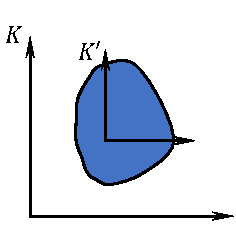
\includegraphics[width=0.6\linewidth]{image/Кинематика Плоского Движения.pdf}
		\subcaption{ }
		\label{fig:12.1.1}
	\end{minipage}
	\hfill
	\begin{minipage}{0.49\linewidth}
		\centering
		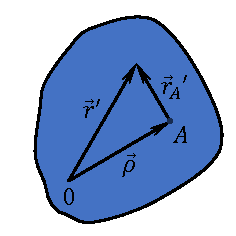
\includegraphics[width=0.6\linewidth]{image/Кинематика Плоского Движения 1.pdf}
		\subcaption{ }
		\label{fig:12.1.2}
	\end{minipage}
	\caption{Иллюстрации к вопросу}
	\label{fig:5}
\end{figure}

Возьмем разные полюса. Будет ли $\omega$ зависеть от выбора полюса?
\begin{align*}
	&\vec{v}=\vec{v}_0+ [\vec{\omega}; \, \vec{r}^{\, \prime}] \\
	&\vec{v}=\vec{v}_A+[\vec{\omega}_A; \, \vec{r}^{\, \prime}_A] \\
	& \vec{v}_0+ [\vec{\omega}; \, \vec{r}^{\, \prime}] = \vec{v}_A+[\vec{\omega}_A; \, \vec{r}^{\, \prime}_A]\\
	&\vec{v}_A = \vec{v}_0 + [\vec{\omega}; \, \vec{\rho}] \text{ -- т.к. точка $A$ вращается вокруг $O$}\\
	& \vec{v}_0+ [\vec{\omega}; \, \vec{r}^{\, \prime}] = \vec{v}_0+[\vec{\omega}; \, \vec{\rho}]+[\vec{\omega}_A; \, \vec{r}^{\, \prime}_A] \\
	& [\vec{\omega}; \, (\vec{r}^{\, \prime} - \vec{\rho})] = \vec{v}_0+[\vec{\omega}; \, \vec{\rho}]+[\vec{\omega}_A; \, \vec{r}^{\, \prime}_A] \\
	& [\vec{\omega}; \, (\vec{r}^{\, \prime} - \vec{\rho})] = [\vec{\omega}_A; \, \vec{r}^{\, \prime}_A] \\
	& \begin{aligned}
		\left.\begin{matrix}
			\vec{r}^{\,\prime} = \vec{\rho} + \vec{r}_A^{\, \prime} \\
			\vec{r}^{\,\prime} - \vec{\rho} = \vec{r}_A^{\,\prime}
		\end{matrix} \, \right|
		\Rightarrow [\vec{\omega}; \, \vec{r}_A^{\,\prime}] = [\vec{\omega}_A; \, \vec{r}_A^{\,\prime}]
	\end{aligned}
\end{align*}

В общем случае $\vec{\omega} \neq \vec{\omega}_A$, но в случае плоского движения $\vec{\omega}_A = \vec{\omega}$.

\textbf{Вывод:} Угловая скорость вращения носит абсолютный характер, то есть можно не указывать ось вращения. Часто за полюс берут центр масс.
\[\vec{v} = \vec{v} + [\vec{\omega}; \, \vec{r}^*]\]
где $\vec{r}^*$ -- радиус-вектор от центра масс до произвольной точки.

\subsubsection*{Мгновенная ось вращения}

\textbf{Мгновенная ось вращения} -- это ось, связанная с точкой тела, у которой скорость равна нулю ($\vec{v} = 0$) в данный момент времени. Такую точку всегда можно найти:
\[\vec{v} = \vec{v}_c + [\vec{\omega}; \, \vec{r}_M^{\,*}] = 0 \, \Big| \cdot \vec{\omega}\]
\[[\vec{\omega}; \, \vec{v}_c] + [\vec{\omega}; \, [\vec{\omega}; \, \vec{r}_M^{\, *}]] = 0\]
\[[\vec{\omega}; \, \vec{v}_c] + \omega\underbrace{(\vec{\omega}; \, \vec{r}_M^{\,*})}_{0} - \vec{r}_M^{\,*} \vec{\omega}^2 = 0\]
\[\begin{aligned}
	\vec{r}_M^{\,*} = \frac{[\vec{\omega}; \, \vec{v}_c]}{\omega^2} &&\to&& \vec{r}_M^{\,*} = \frac{v_c}{\omega}
\end{aligned}\]

\textbf{Пример:} Цилиндр без проскальзывания движется по плоскости. (см. рис. \ref{fig:7}) \textbf{Важно!} Понятие Мгновенной Оси Вращения нельзя использовать для поиска распределения ускорения.
\begin{figure}[H]
	\centering
	\includegraphics[width=0.6\linewidth]{"image/Кинематика Плоского Движения 3"}
	\caption{Пример}
	\label{fig:7}
\end{figure}


